\documentclass[a4paper, 12pt]{article}
\usepackage[utf8x]{inputenc}
\usepackage{cmap}
\usepackage[english, russian]{babel}
\usepackage{indentfirst}
\usepackage[left=20mm, top=20mm, right=20mm, bottom=20mm]{geometry}
\usepackage{tikz}
\usepackage{float}
\usepackage{amsmath, amsfonts, amssymb}
\usepackage{graphicx}
\usepackage{fancybox, fancyhdr}
\usepackage{hyperref}
\usepackage{listings}
\usepackage{caption}
\usepackage{subcaption}
\usepackage{xcolor}
\usepackage{paralist}
\pagestyle{fancy}
\fancyhf{}
\fancyhead[L]{Лабораторная работа №7}
\fancyhead[R]{Линейные системы автоматического управления}
\fancyfoot[C]{\thepage}
\graphicspath{{images/}}
\usetikzlibrary{patterns}
\definecolor{LightGray}{gray}{0.95}
\definecolor{LightGray2}{gray}{0.7}
\hypersetup{
    colorlinks=true,
    linkcolor=blue,
    filecolor=magenta,
    urlcolor=cyan,
    pdftitle={contents setup},
    pdfpagemode=FullScreen,
}
\setlength{\parskip}{1.5mm}
\setlength{\headheight}{15pt}
\setlength{\footskip}{15pt}
\allowdisplaybreaks

\begin{document}
    \begin{titlepage}

        \begin{center}
        
\includegraphics[width=0.3\textwidth]{itmo.png} % requires itmo.png in /images folder
        \vfill
        
        Федеральное государственное автономное образовательное учреждение высшего образования
        «Национальный Исследовательский Университет ИТМО»\\
        
        \vfill
        {\large\bf ЛАБОРАТОРНАЯ РАБОТА №6}\\
        {\large\bf ПРЕДМЕТ «ЛИНЕЙНЫЕ СИСТЕМЫ АВТОМАТИЧЕСКОГО УПРАВЛЕНИЯ»}\\
        {\large\bf ТЕМА «АНАЛИЗ ТОЧНОСТИ СИСТЕМ УПРАВЛЕНИЯ»}\\
        Вариант 4
        \vfill

        \begin{flushright}
            \begin{minipage}{.45\textwidth}
            {
                \hbox{Преподаватель: Золотаревич В. П.}
                \hbox{Студент: Румянцев А. А.}
                \hbox{Поток: ЛСАУ R22 бак 4.1.1}
                \hbox{}
                \hbox{Факультет: СУиР}
                \hbox{Группа: R3341}
            }
            \end{minipage}
        \end{flushright}
        
        \vfill
                
        Санкт-Петербург\\
        2024
        \end{center}
    \end{titlepage}
    
    \tableofcontents

    \newpage
    \section{Цель работы}
    Исследование точностных свойств систем управления.


    \section{Задание 1}
    \subsection{Условие}
    \textit{Исследование системы с астатизмом нулевого порядка.}
    \begin{compactitem}
        \item Структура системы представлена на рис. \ref{fig:struct_scheme1}, где $H(s)=k$. Передаточная функции объекта
        управления $$W(s)=\dfrac{1.5}{s^2+2s+1},$$ характеристики задающего воздействия $g(t):1,t$
        \begin{figure}[H]
            \centering
            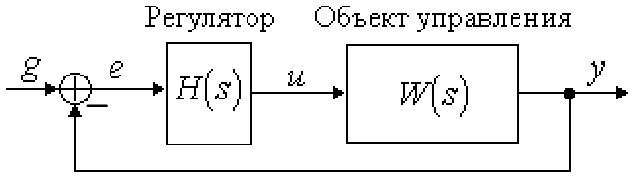
\includegraphics[scale=0.7]{struct_scheme1.png}
            \captionsetup{skip=0pt}
            \caption{Схема эксперимента}
            \label{fig:struct_scheme1}
        \end{figure}
        \item Исследование стационарного режима работы: $g(t)=A$.
        Получить переходные процессы для трех различных значений
        коэффициента $k$ и определить предельное
        значение установившейся ошибки $\varepsilon$.
        Значения коэффициента $k$ (здесь и во
        всех последующих пунктах): $1, 5, 10$.
        \item Исследование режима движения
        с постоянной скоростью: $g(t)=Vt$.
        Получить переходные процессы для различных
        значений коэффициента $k$. Интервал наблюдения --
        $30$ секунд.
    \end{compactitem}
     

    \subsection{Выполнение}
    Схема моделирования при $g(t)=A$ и при $g(t)=Vt$ представлена на рис. \ref{fig:scheme1}.
    Заданные параметры блока ``Transfer Fcn'' находятся на рис. \ref{fig:task1_tfcn_window}
    под заголовком <<Приложения>>.
    \begin{figure}[H]
        \centering
        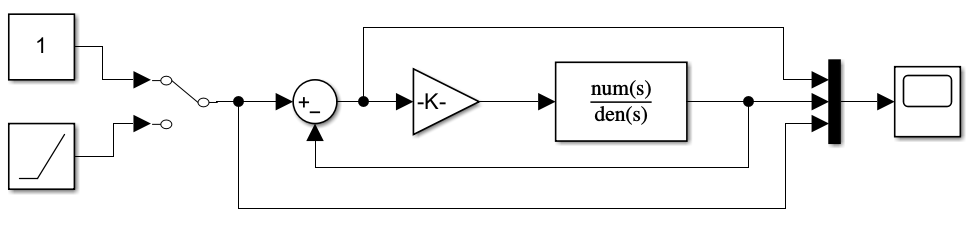
\includegraphics[scale=0.6]{scheme1.png}
        \captionsetup{skip=0pt}
        \caption{Схема эксперимента}
        \label{fig:scheme1}
    \end{figure}


    Рассмотрим $g(t)=A$. Рассчитаем предельное значение установившейся ошибки
    $$\varepsilon=\lim\limits_{s\rightarrow0}s\dfrac{1}{1+W(s)}\dfrac{A}{s}=\dfrac{A}{1+k}$$
    При $A=1$ получаем
    $$
    \begin{matrix}
        k=1:\ \ \, \varepsilon=1/(1+1)=1/2\\
        k=5:\ \ \, \varepsilon=1/(1+5)=1/6\\
        k=10:\ \varepsilon=1/(1+10)=1/11
    \end{matrix}
    $$
    Построим графики переходных процессов (реакции системы) при $g(t)=A$ и различных $k$. Синий график -- $y(t)$, желтый -- $e(t)$, оранжевый -- $g(t)$.
    \begin{figure}[H]
        \centering
        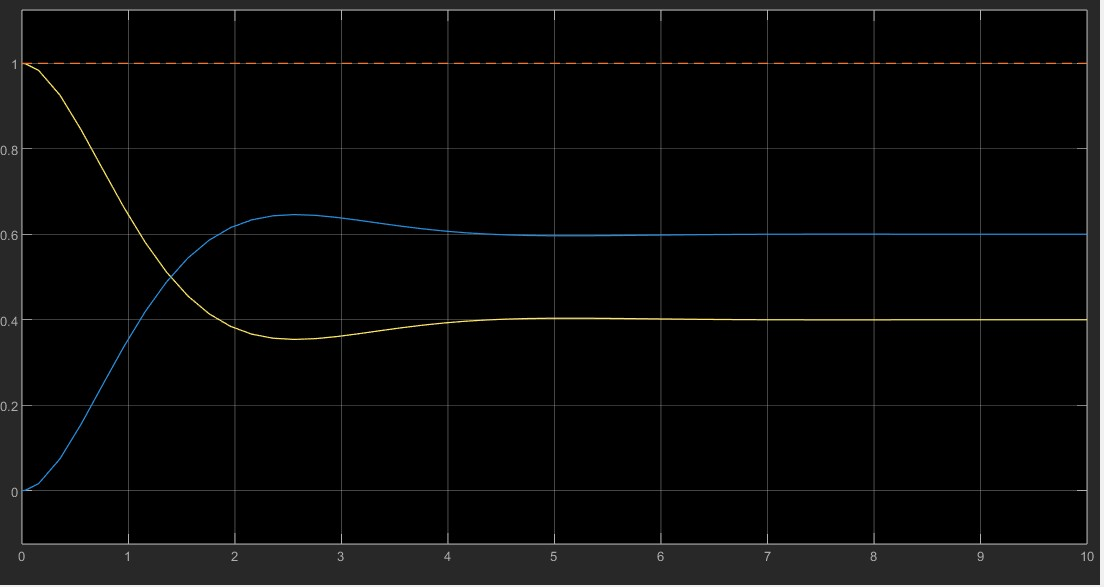
\includegraphics[scale=0.3]{task_1_g=1_k=1.jpg}
        \captionsetup{skip=0pt}
        \caption{Переходный процесс при $g(t)=1,k=1$}
        \label{fig:t1g1k1}
    \end{figure}
    \begin{figure}[H]
        \centering
        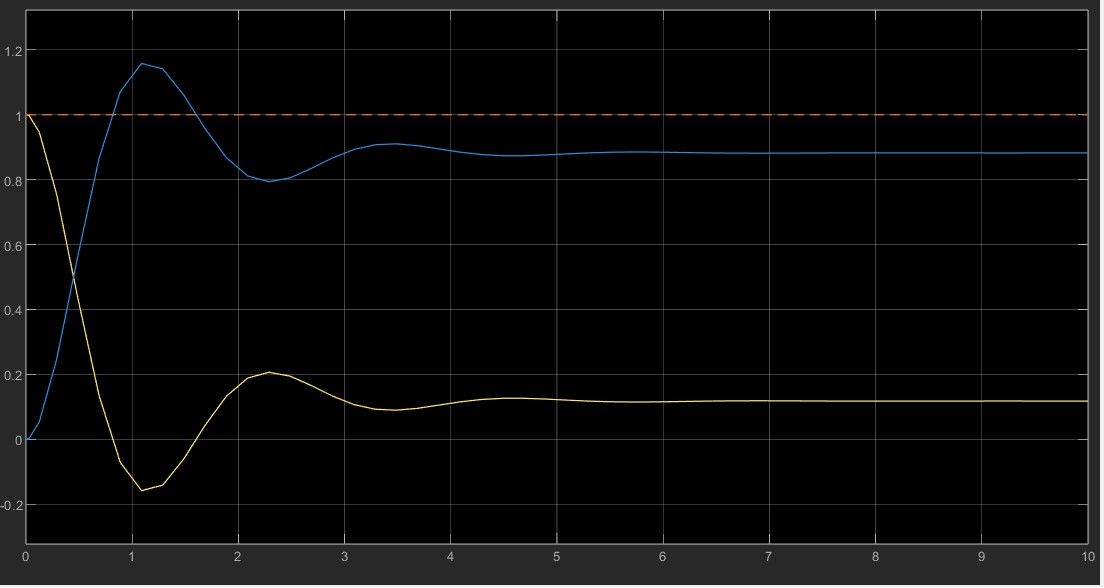
\includegraphics[scale=0.3]{task_1_g=1_k=5.jpg}
        \captionsetup{skip=0pt}
        \caption{Переходный процесс при $g(t)=1,k=5$}
        \label{fig:t1g1k5}
    \end{figure}
    \begin{figure}[H]
        \centering
        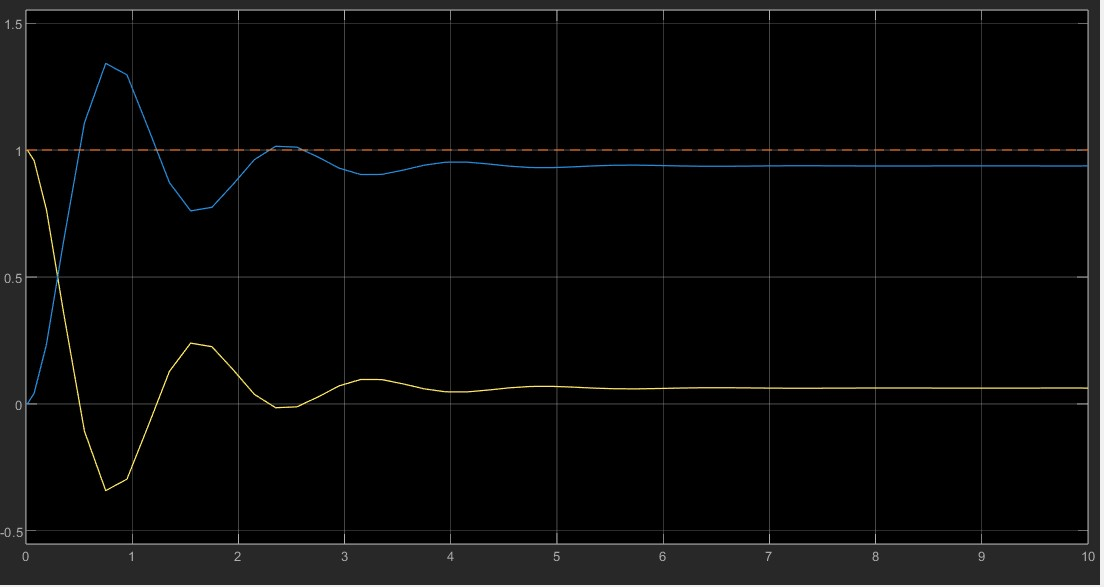
\includegraphics[scale=0.3]{task_1_g=1_k=10.jpg}
        \captionsetup{skip=0pt}
        \caption{Переходный процесс при $g(t)=1,k=10$}
        \label{fig:t1g1k10}
    \end{figure}
    Рассмотрим $g(t)=Vt=t$. Рассчитаем предельное значение установившейся ошибки.
    При линейно нарастающем входном воздействии имеем
    $$\varepsilon=\lim\limits_{s\rightarrow0}s\dfrac{1}{1+W(s)}\dfrac{V}{s^2}=\dfrac{1}{1+k}\dfrac{V}{s}=\infty,$$
    следовательно, линейно возрастающее задающее воздействие отрабатывается
    статической системой с неограниченно растущей ошибкой при любых $k$: $\varepsilon_k=\infty,\forall k$. Построим графики.
    \begin{figure}[H]
        \centering
        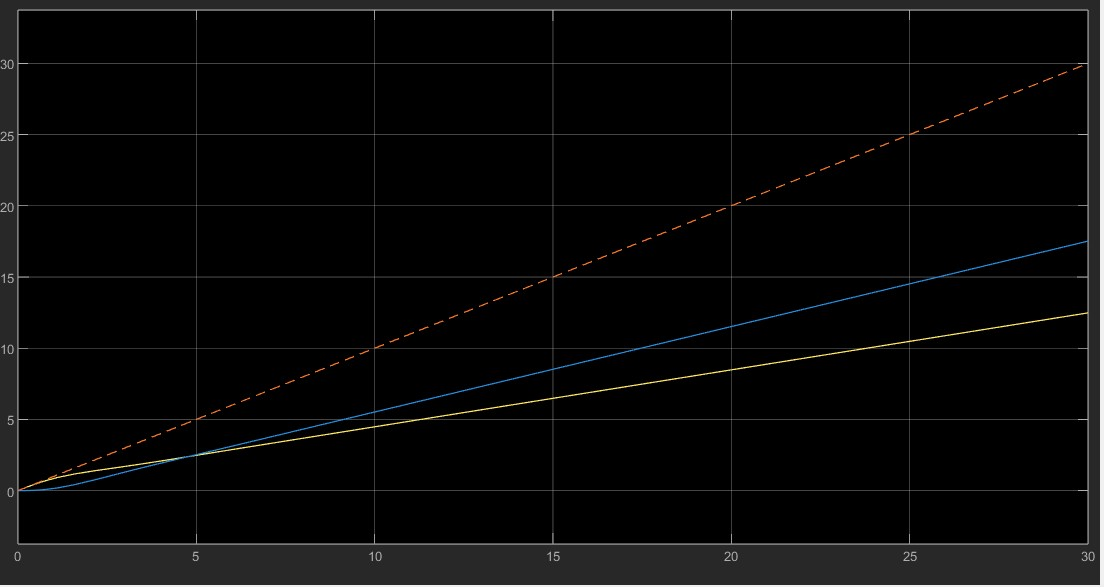
\includegraphics[scale=0.3]{task_1_g=t_k=1.jpg}
        \captionsetup{skip=0pt}
        \caption{Переходный процесс при $g(t)=t,k=1$}
        \label{fig:t1gtk1}
    \end{figure}
    \begin{figure}[H]
        \centering
        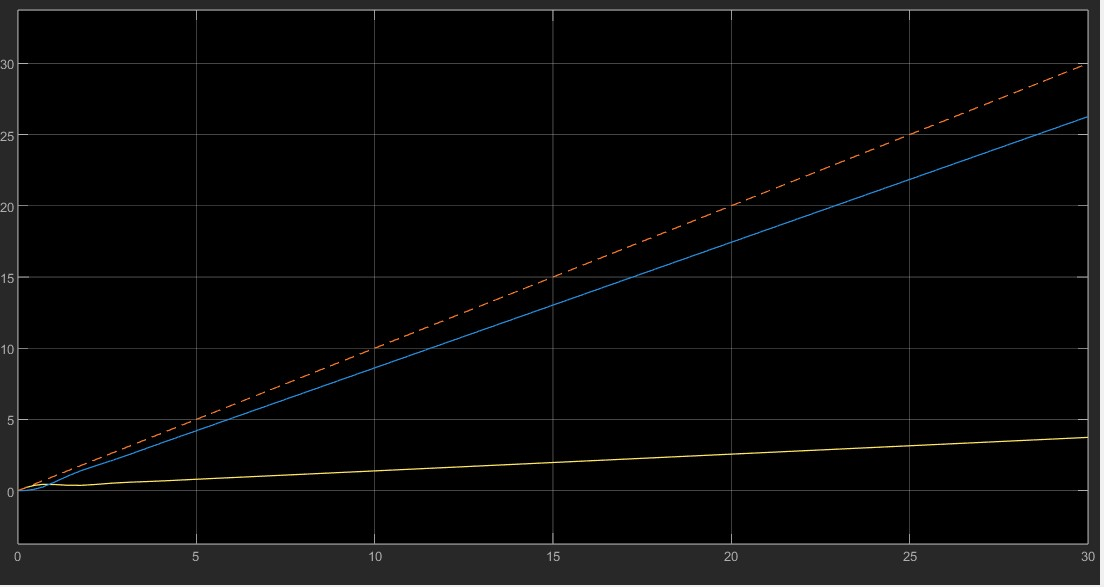
\includegraphics[scale=0.3]{task_1_g=t_k=5.jpg}
        \captionsetup{skip=0pt}
        \caption{Переходный процесс при $g(t)=t,k=5$}
        \label{fig:t1gtk5}
    \end{figure}
    \begin{figure}[H]
        \centering
        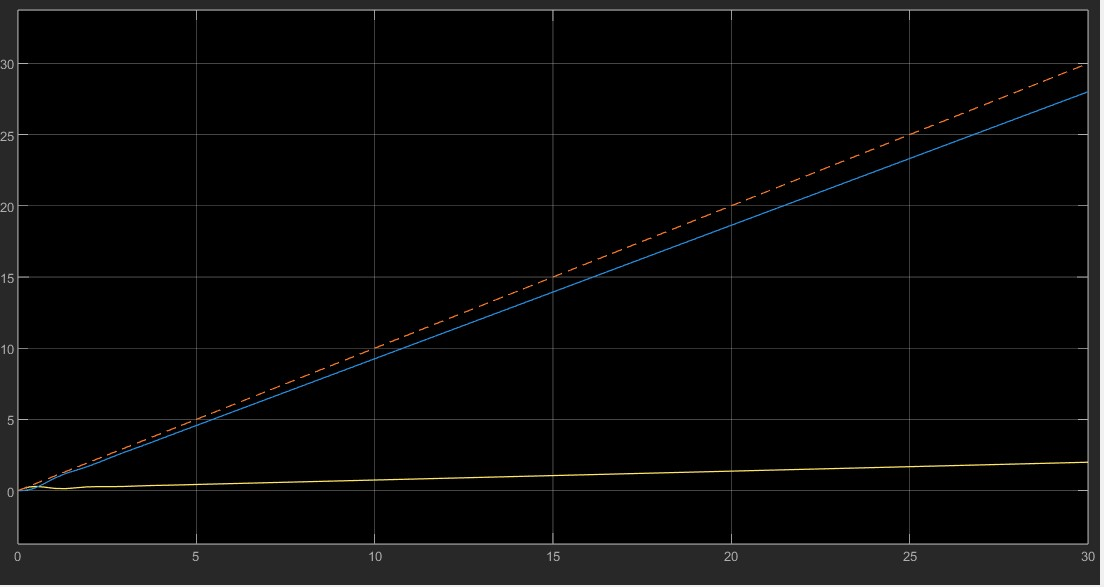
\includegraphics[scale=0.3]{task_1_g=t_k=10.jpg}
        \captionsetup{skip=0pt}
        \caption{Переходный процесс при $g(t)=t,k=10$}
        \label{fig:t1gtk10}
    \end{figure}
    

    \section{Задание 2}
    \subsection{Условие}
    \textit{Исследование системы с астатизмом первого порядка.}
    \begin{compactitem}
    \item Структура системы представлена на рис. \ref{fig:struct_scheme1}, где
    $H(s)=k/s$. Передаточная функция объекта управления $$W(s)=\dfrac{s+1.5}{s^2+2s+1},$$
    характеристики квадратично нарастающего задающего воздействия $$g(t)=\dfrac{at^2}{2}=0.4t^2$$
    Характеристики постоянного и линейно нарастающего задающих воздействий взять из задания 1.
    \item Исследование стационарного режима работы: $g(t)=A$.
    Получить переходные процессы для различных значений коэффициента $k$ и определить предельное
    значение установившейся ошибки $\varepsilon$.
    \item Исследование режима движения с постоянной скоростью: $g(t)=Vt$.
    Получить переходные процессы для различных значений коэффициента $k$ и определить
    предельное значение установившейся ошибки $\varepsilon$. Интервал наблюдения -- $30$ секунд.
    \item Исследование режима движения с постоянным ускорением: $g(t)=at^2/2$.
    Получить переходные процессы для различных значений коэффициента $k$. Интервал
    наблюдения -- $30$ секунд.
    \end{compactitem}


    \subsection{Выполнение}
    Схема моделирования системы для исследования стационарного режима $g(t)=A$ и режима движения $g(t)=Vt$ представлена на рис. \ref{fig:scheme2_1_2}.
    Параметры SIMULINK блока ``Transfer Fcn'' на рис. \ref{fig:task2_tfcn_window} под заголовком <<Приложения>>.
    \begin{figure}[H]
        \centering
        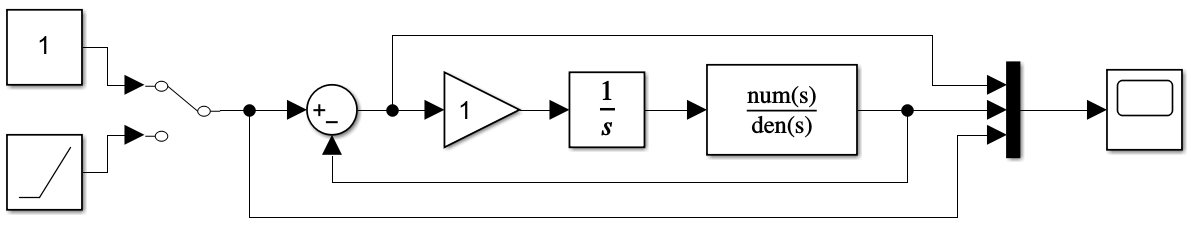
\includegraphics[scale=0.6]{scheme2_1_2.png}
        \captionsetup{skip=0pt}
        \caption{Схема эксперимента}
        \label{fig:scheme2_1_2}
    \end{figure}


    Рассмотрим $g(t)=A$. Рассчитаем предельное значение установившейся ошибки.
    Для системы с первым порядком астатизма при постоянном входном воздействии используем
    $$\varepsilon=\lim\limits_{s\rightarrow0}s\dfrac{1}{1+W(s)}\dfrac{A}{s}=\lim\limits_{s\rightarrow0}\dfrac{1}{1+\dfrac{W^*(s)}{s}}A=\lim\limits_{s\rightarrow0}\dfrac{s}{s+k}A=0,$$
    то есть $\varepsilon_k=0,\forall k$. Построим графики переходных процессов при различных $k$ для $g(t)=A$. Синий график -- $y(t)$, желтый -- $e(t)$, оранжевый -- $g(t)$.
    \begin{figure}[H]
        \centering
        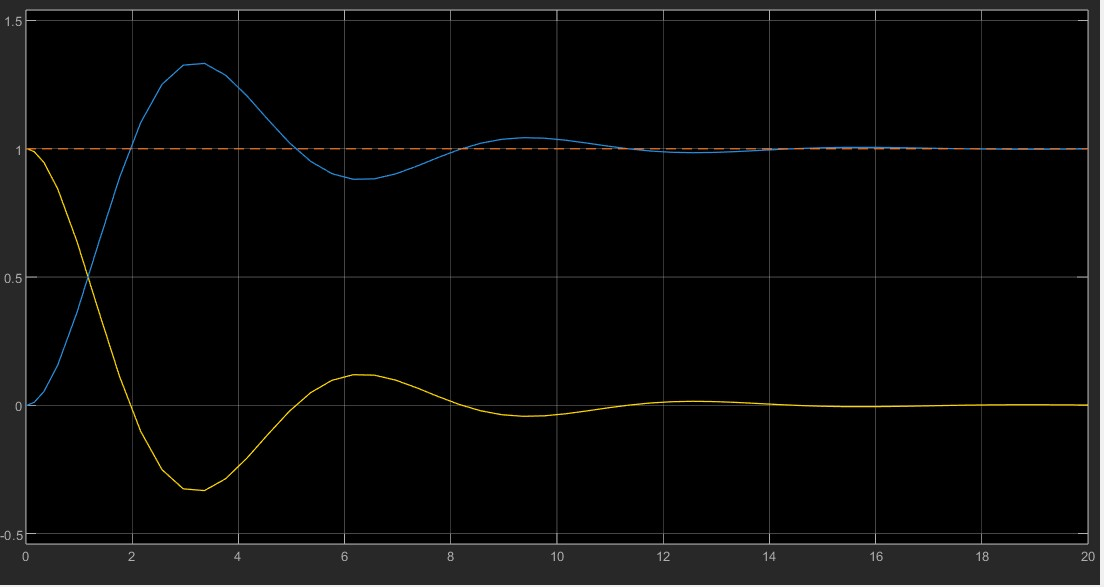
\includegraphics[scale=0.3]{task_2_g=1_k=1.jpg}
        \captionsetup{skip=0pt}
        \caption{Переходный процесс при $g(t)=1,k=1$}
        \label{fig:t2g1k1}
    \end{figure}
    \begin{figure}[H]
        \centering
        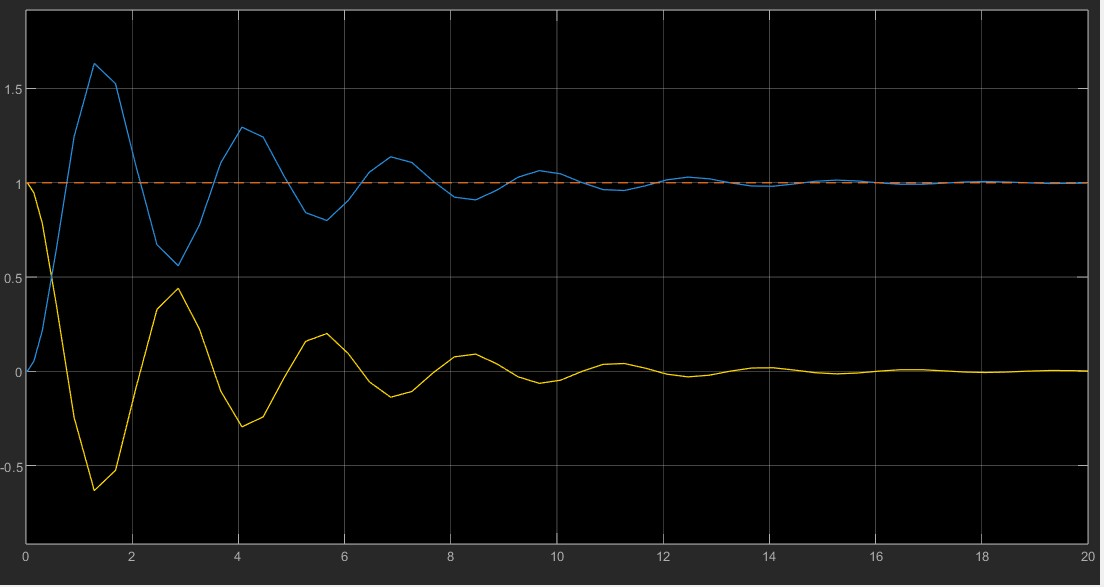
\includegraphics[scale=0.3]{task_2_g=1_k=5.jpg}
        \captionsetup{skip=0pt}
        \caption{Переходный процесс при $g(t)=1,k=5$}
        \label{fig:t2g1k5}
    \end{figure}
    \begin{figure}[H]
        \centering
        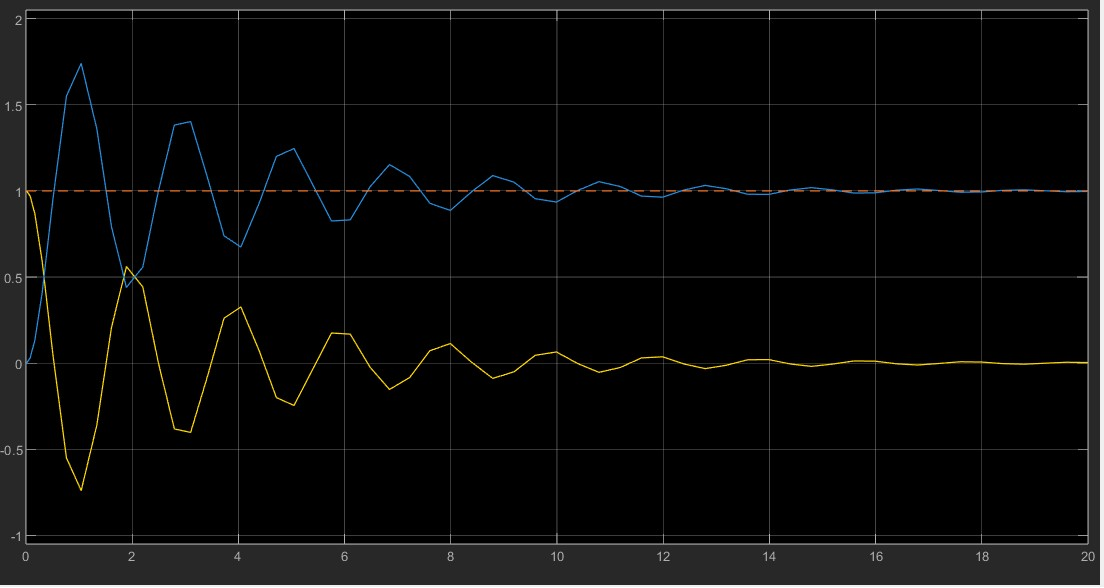
\includegraphics[scale=0.3]{task_2_g=1_k=10.jpg}
        \captionsetup{skip=0pt}
        \caption{Переходный процесс при $g(t)=1,k=10$}
        \label{fig:t2g1k10}
    \end{figure}


    Рассмотрим $g(t)=Vt=t$. Рассчитаем предельное значение установившейся ошибки.
    Для системы с первым порядком астатизма при линейно нарастающем воздействии используем
    $$\varepsilon=\lim\limits_{s\rightarrow0}s\dfrac{1}{1+W(s)}\dfrac{V}{s^2}=\lim\limits_{s\rightarrow0}\dfrac{s}{s+k}\dfrac{V}{s}=\dfrac{V}{k}
    \Rightarrow\text{При } V=1:\ \begin{matrix}
        k=1:\varepsilon=1/1=1\\
        k=5:\ \ \ \ \ \,\varepsilon=1/5\\
        k=10:\ \ \ \ \ \,\varepsilon=1/10
    \end{matrix}$$
    Аналогично построим графики.
    \begin{figure}[H]
        \centering
        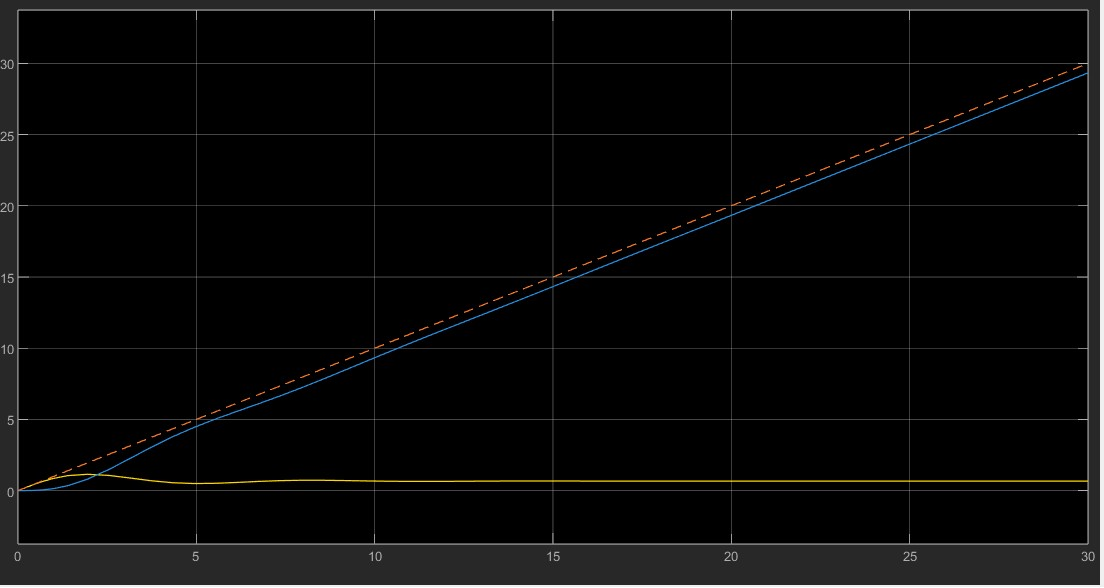
\includegraphics[scale=0.3]{task_2_g=t_k=1.jpg}
        \captionsetup{skip=0pt}
        \caption{Переходный процесс при $g(t)=t,k=1$}
        \label{fig:t2gtk1}
    \end{figure}
    \begin{figure}[H]
        \centering
        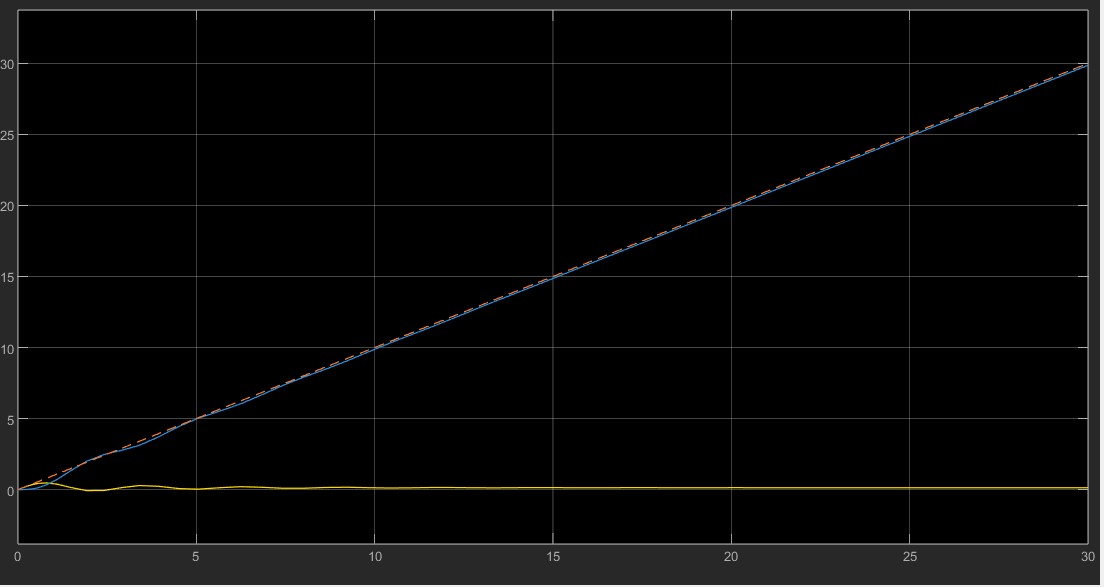
\includegraphics[scale=0.3]{task_2_g=t_k=5.jpg}
        \captionsetup{skip=0pt}
        \caption{Переходный процесс при $g(t)=t,k=5$}
        \label{fig:t2gtk5}
    \end{figure}
    \begin{figure}[H]
        \centering
        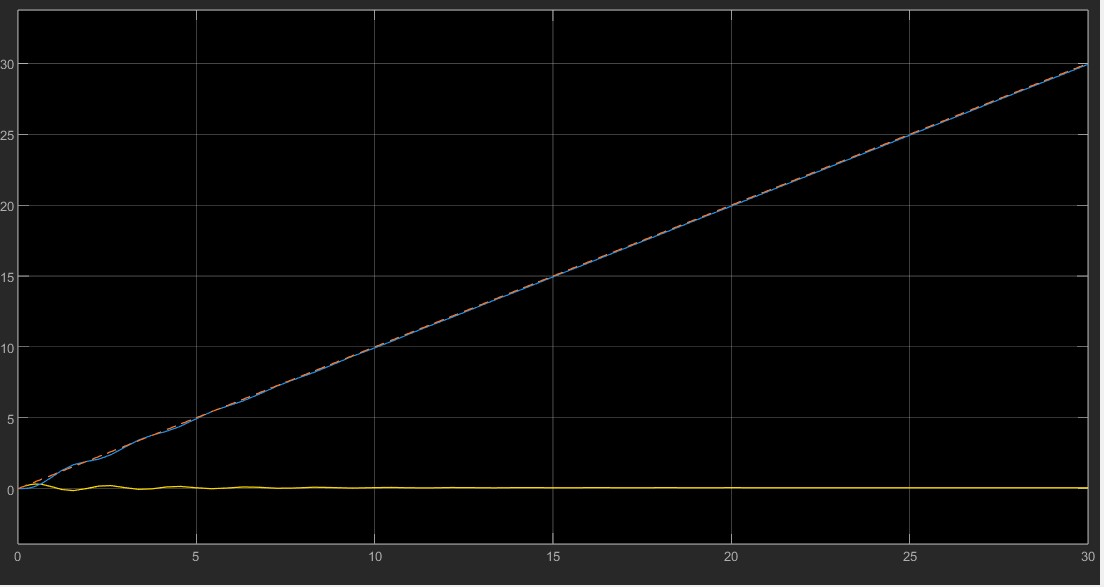
\includegraphics[scale=0.3]{task_2_g=t_k=10.jpg}
        \captionsetup{skip=0pt}
        \caption{Переходный процесс при $g(t)=t,k=10$}
        \label{fig:t2gtk10}
    \end{figure}


    Рассмотрим $g(t)=at^2/2=0.4t^2$. Схема моделирования системы для исследования движения
    с постоянным ускорением представлена на рис. \ref{fig:scheme2_3}
    \begin{figure}[H]
        \centering
        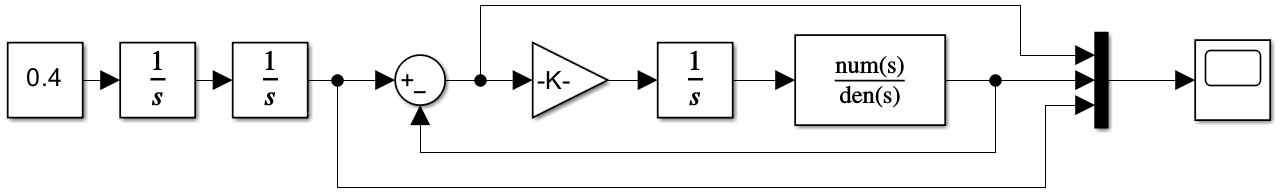
\includegraphics[scale=0.6]{scheme2_3.png}
        \captionsetup{skip=0pt}
        \caption{Схема эксперимента}
        \label{fig:scheme2_3}
    \end{figure}
    \noindent Рассчитаем предельное значение установившейся ошибки.
    Для системы с первым порядком астатизма при квадратично возрастающем воздействии имеем (см. методическое пособие)
    $$\varepsilon_k=\infty,\forall k$$
    Построим графики аналогично.
    \begin{figure}[H]
        \centering
        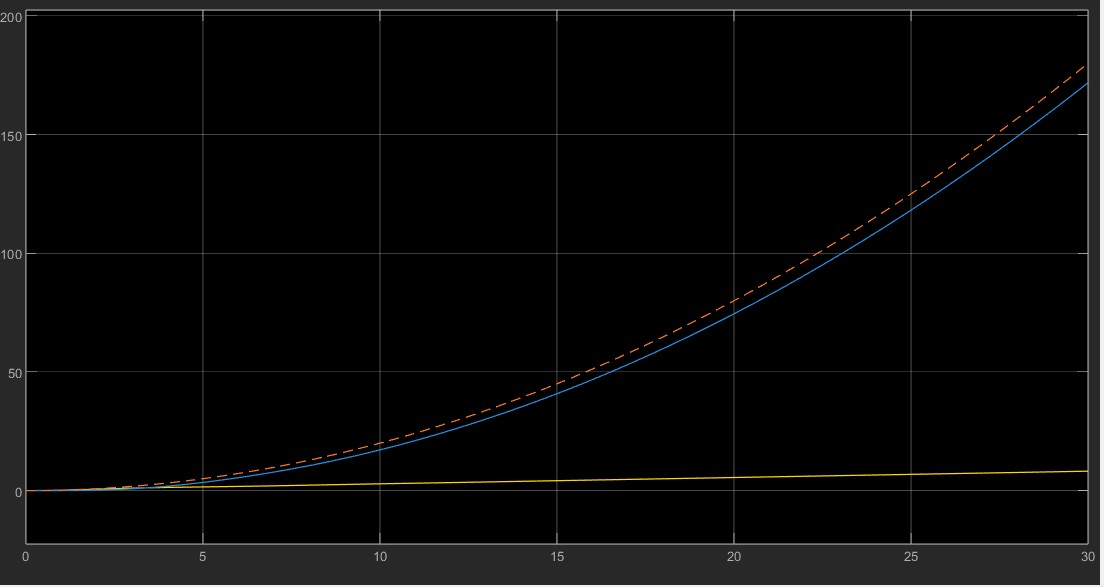
\includegraphics[scale=0.3]{task_2_g=at2_k=1.jpg}
        \captionsetup{skip=0pt}
        \caption{Переходный процесс при $g(t)=at^2/2,k=1$}
        \label{fig:t2gat2k1}
    \end{figure}
    \vspace{15mm}
    \begin{figure}[H]
        \centering
        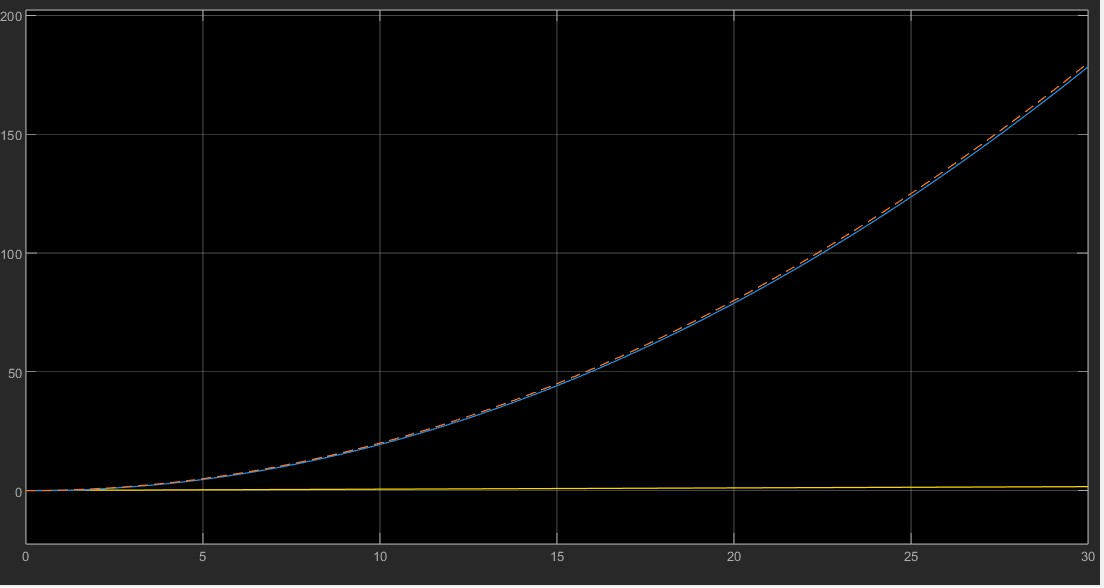
\includegraphics[scale=0.3]{task_2_g=at2_k=5.jpg}
        \captionsetup{skip=0pt}
        \caption{Переходный процесс при $g(t)=at^2/2,k=5$}
        \label{fig:t2gat2k5}
    \end{figure}
    \begin{figure}[H]
        \centering
        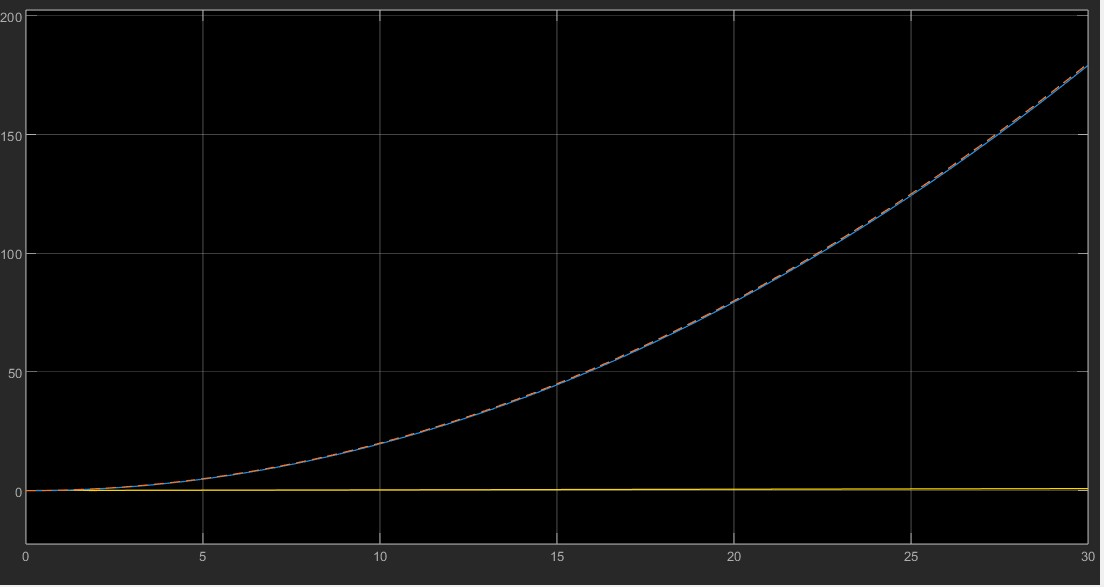
\includegraphics[scale=0.3]{task_2_g=at2_k=10.jpg}
        \captionsetup{skip=0pt}
        \caption{Переходный процесс при $g(t)=at^2/2,k=10$}
        \label{fig:t2gat2k10}
    \end{figure}


    \section{Задание 3}
    \subsection{Условие}
    \textit{Исследование влияния внешних возмущений.}
    \begin{compactitem}
        \item Cобрать схему моделирования возмущенной системы. Дано:
        $$W(s)=\dfrac{1.5}{s^2+2s+1},\ \ f_1(t)=2,\ \ f_2(t)=1$$
        Структура системы представлена на рис. \ref{fig:struct_scheme3}.
        \begin{figure}[H]
            \centering
            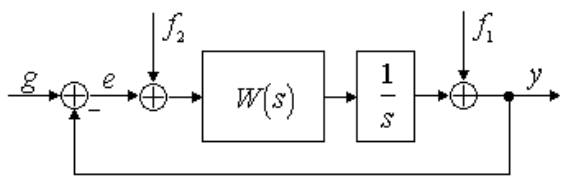
\includegraphics[scale=0.75]{struct_scheme3.png}
            \captionsetup{skip=0pt}
            \caption{Схема эксперимента}
            \label{fig:struct_scheme3}
        \end{figure}
        \item Полагая $f_2(t)\equiv0$ и $g(t)=1(t)$, получить переходной процесс и определить
        предельное значение установившейся ошибки $\varepsilon$.
        \item Полагая $f_1(t)\equiv0$ и $g(t)=1(t)$, получить переходной процесс и определить
        предельное значение установившейся ошибки $\varepsilon$.
    \end{compactitem}


    \subsection{Выполнение}
    Рассмотрим $f_2(t)\equiv0$ и $g(t)=1(t)$. Схема моделирования возмущенной системы
    представлена на рис. \ref{fig:scheme3_1}.
    \begin{figure}[H]
        \centering
        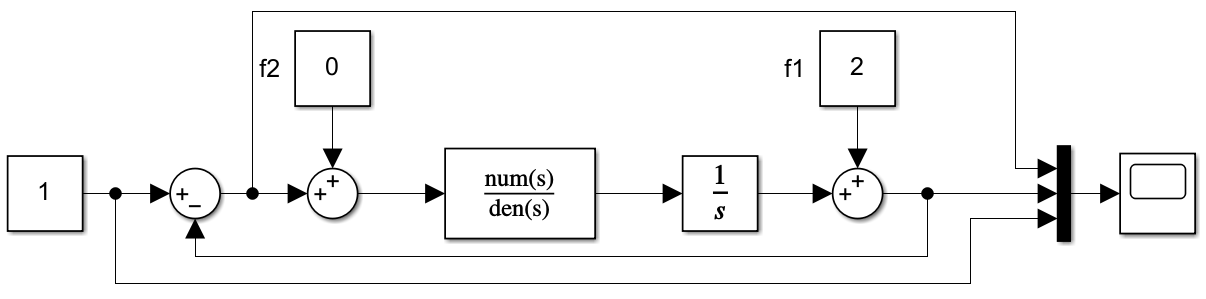
\includegraphics[scale=0.6]{scheme3_1.png}
        \captionsetup{skip=0pt}
        \caption{Схема эксперимента}
        \label{fig:scheme3_1}
    \end{figure}
    \noindent Рассчитаем предельное значение установившейся ошибки. Из методического пособия имеем расчет ошибки в общем виде
    $$e=g-y=-y=-W(s)\left(f_1-\dfrac{1}{s}\left(f_2+y\right)\right)=-W(s)\left(f_1-\dfrac{1}{s}\left(f_2-e\right)\right),$$
    что можно записать как
    $$\left(1+\dfrac{1}{s}W(s)\right)e=-W(s)f_1+\dfrac{1}{s}W(s)f_2$$
    После элементарных преобразований получаем
    $$e=-\dfrac{W(s)}{1+\dfrac{1}{s}W(s)}f_1+\dfrac{\dfrac{1}{s}W(s)}{1+\dfrac{1}{s}W(s)}f_2=-\dfrac{sW(s)}{s+W(s)}f_1+\dfrac{W(s)}{s+W(s)}f_2$$
    Пусть возмущения $f_1(t)=F_1$ и $f_2(t)=F_2$ являются постоянными, тогда
    $$\varepsilon=\lim\limits_{s\rightarrow0}\left[-s\dfrac{sW(s)}{s+W(s)}\dfrac{F_1}{s}+s\dfrac{W(s)}{s+W(s)}\dfrac{F_2}{s}\right]=F_2$$
    Таким образом, возмущение $f_2$ дает статическую ошибку (величина которой не
    зависит от параметров системы управления), а влияние возмущения $f_1$ полностью компенсировано.
    Так как мы положили $f_2(t)\equiv0$, следовательно $$\varepsilon=f_2(t)=0$$
    Построим график переходного процесса. Синий -- $y(t)$, желтый -- $e(t)$, оранжевый -- $g(t)$.
    Видим, что ошибка стабилизируется к значению 0.
    \begin{figure}[H]
        \centering
        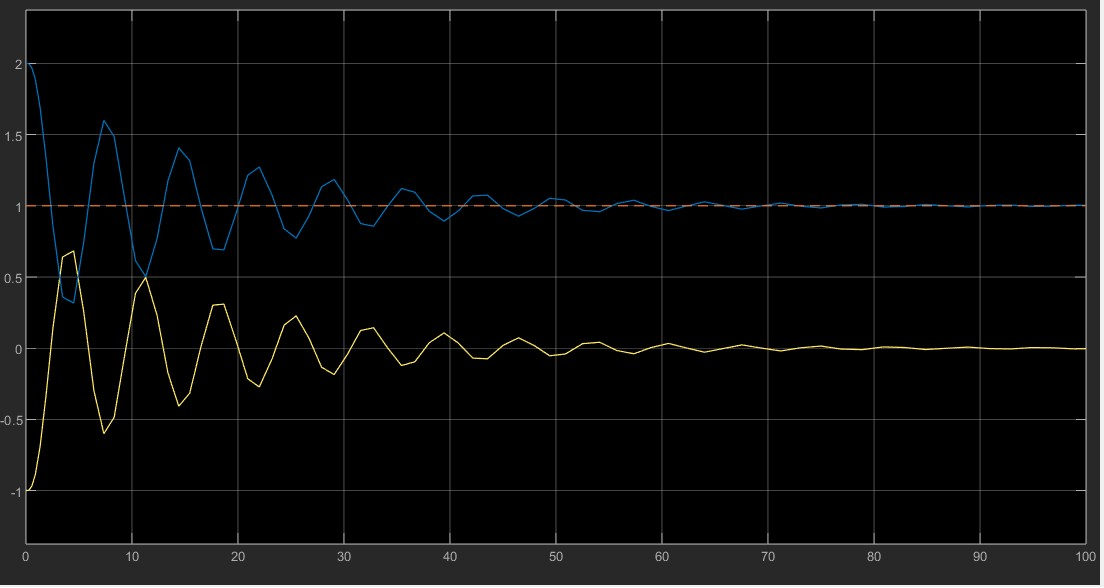
\includegraphics[scale=0.3]{task_3_f2=0.jpg}
        \captionsetup{skip=0pt}
        \caption{Переходный процесс при $f_2(t)\equiv0,g(t)=1(t)$}
        \label{fig:t3f2eq0}
    \end{figure}


    Рассмотрим $f_1(t)\equiv0$ и $g(t)=1(t)$. Схема моделирования возмущенной системы
    представлена на рис. \ref{fig:scheme3_2}.
    \begin{figure}[H]
        \centering
        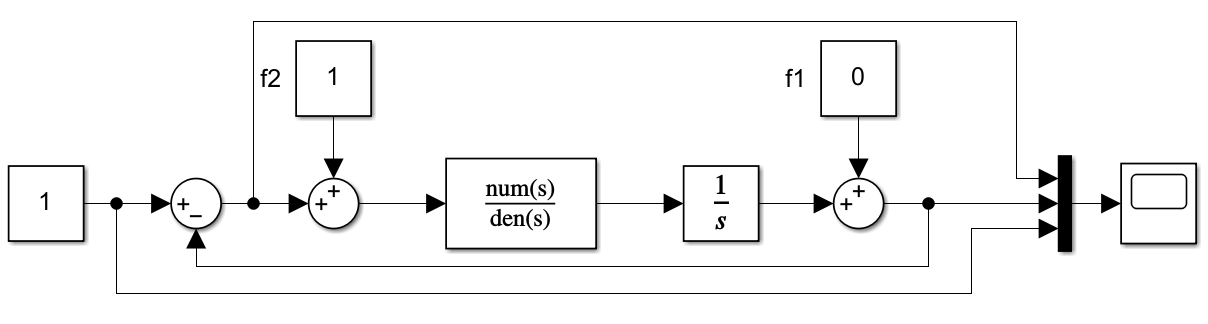
\includegraphics[scale=0.6]{scheme3_2.png}
        \captionsetup{skip=0pt}
        \caption{Схема эксперимента}
        \label{fig:scheme3_2}
    \end{figure}
    \noindent Расчет ошибки аналогичен, следовательно
    $$\varepsilon=f_2(t)=1$$
    Аналогично построим график. Желтый график ошибки стабилизируется к $1=\varepsilon$.
    \begin{figure}[H]
        \centering
        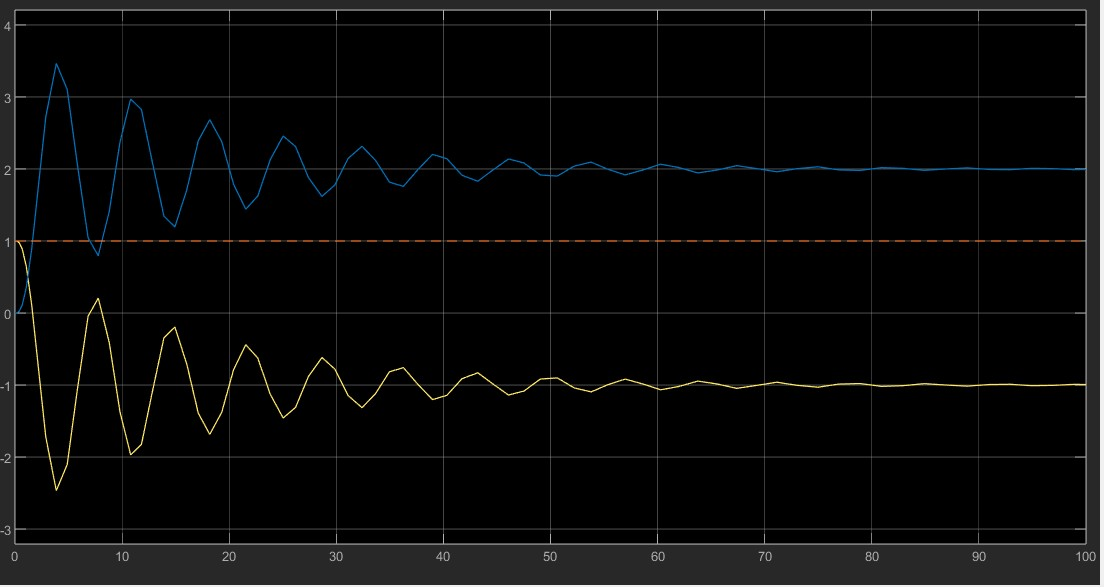
\includegraphics[scale=0.3]{task_3_f1=0.jpg}
        \captionsetup{skip=0pt}
        \caption{Переходный процесс при $f_1(t)\equiv0,g(t)=1(t)$}
        \label{fig:t3f1eq0}
    \end{figure}


    \section{Задание 4}
    \subsection{Условие}
    \textit{Исследование установившейся ошибки при произвольном входном воздействии.}
    Структура системы представлена на рис. \ref{fig:struct_scheme1}, где $H(s)=1$. Дано:
    $$W(s)=\dfrac{1.5}{s^2+2s+1},\ \ g(t)=0.4t+0.2t^2$$
    \begin{compactitem}
    \item Получить переходной процесс в замкнутой системе
    и определить (по графику) установившуюся ошибку слежения $e_y(t)$.
    \item Получить приближенное аналитическое выражение для $e_y(t)$, сохранив в
    ряде Тейлора $$e_y(t)=c_0g(t)+c_1\dfrac{d}{dt}g(t)+\dfrac{c^2}{2!}\dfrac{d^2}{dt^2}g(t)+\dfrac{c^3}{3!}\dfrac{d^3}{dt^3}g(t)...,$$
    где $c_i$ -- коэффициенты ошибок, три первых члена. Построить график $e_y(t)$
    в соответствии с полученным аналитическим выражением (использовать для этого блок нелинейных функций Fnc).
    \end{compactitem}


    \subsection{Выполнение}
    Схема моделирования замкнутой системы представлена на рисунке \ref{fig:scheme4_1}.
    \begin{figure}[H]
        \centering
        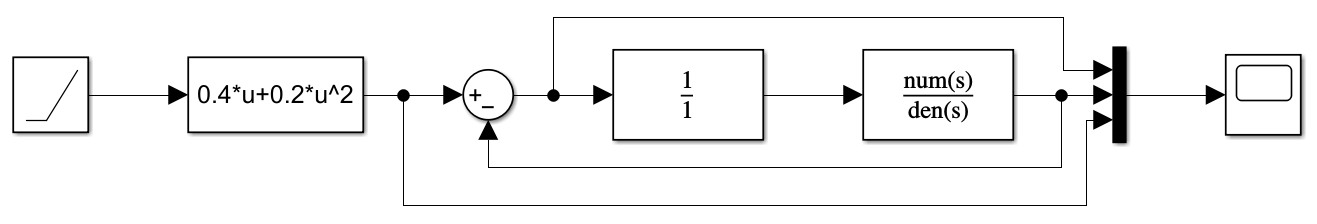
\includegraphics[scale=0.6]{scheme4_1.png}
        \captionsetup{skip=0pt}
        \caption{Схема эксперимента}
        \label{fig:scheme4_1}
    \end{figure}
    \begin{figure}[H]
        \centering
        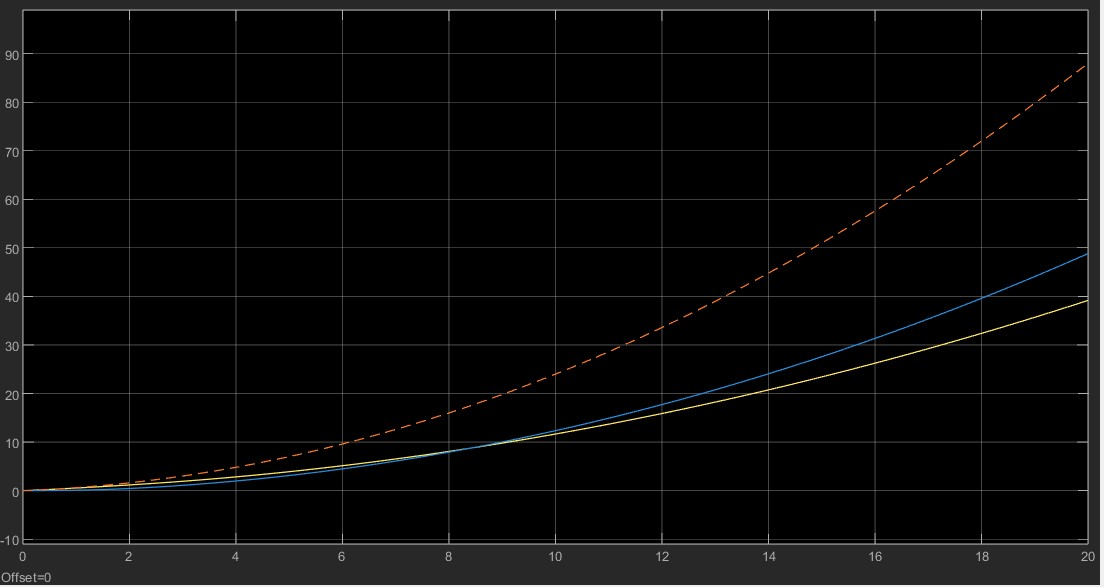
\includegraphics[scale=0.3]{task_4_1.jpg}
        \captionsetup{skip=0pt}
        \caption{Переходный процесс при $g(t)=0.4t+0.2t^2$}
        \label{fig:task_4_1}
    \end{figure}


    \section{Вывод}
    В этой работе мы определяли установившуюся ошибку системы
    по её передаточной функции и сравнивали полученные результаты
    с аналитическим расчетом, подтвердив их совпадение.
    Проведённые исследования продемонстрировали,
    что наличие или отсутствие установившейся ошибки
    следует оценивать для каждого возмущающего воздействия
    на систему, анализируя соответствующие передаточные
    функции от возмущения к ошибке, независимо от порядка
    астатизма системы по задающему воздействию.


    \section{Приложения}
    \begin{figure}[H]
        \centering
        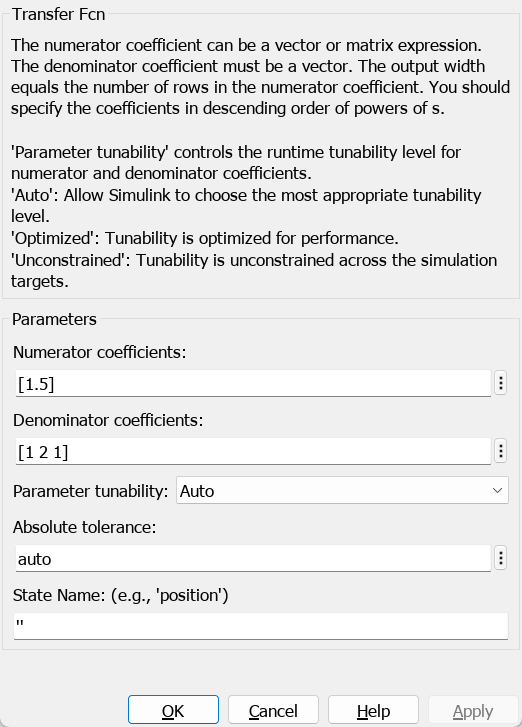
\includegraphics[scale=0.6]{task1_tfcn_window.png}
        \captionsetup{skip=0pt}
        \caption{Параметры SIMULINK для $W(s)=1.5/(s^2+2s+1)$}
        \label{fig:task1_tfcn_window}
    \end{figure}
    \begin{figure}[H]
        \centering
        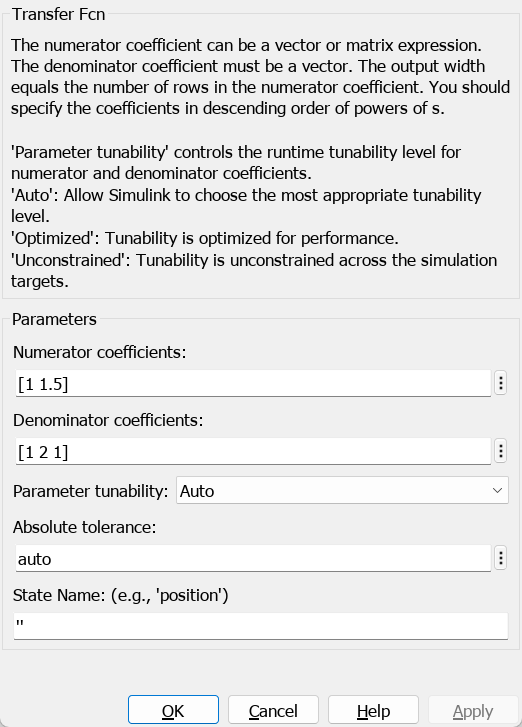
\includegraphics[scale=0.6]{task2_tfcn_window.png}
        \captionsetup{skip=0pt}
        \caption{Параметры SIMULINK для $W(s)=(s+1.5)/(s^2+2s+1)$}
        \label{fig:task2_tfcn_window}
    \end{figure}
\end{document}